\documentclass[a4paper,10pt]{article}
\usepackage[utf8]{inputenc}
\usepackage{amsmath}
\usepackage{graphicx}
\usepackage[english]{babel}
%\usepackage{url}
\usepackage{epstopdf}
%\usepackage{subfig}
\usepackage{graphicx}
\usepackage{enumerate}
%\usepackage{appendix}
%\usepackage{anysize}
%\marginsize{1cm}{1cm}{1cm}{1cm}

\title{\textit{IEE3853} Detectores para Astronomía (I-2012)}
\author{\textbf{Tarea 04 – Diseño del sistema de detección para un Imager} \\Norman F. Sáez\\nfsaez@uc.cl}

\date{2012/07/07}

\begin{document}
\maketitle
\section[1]{Introducción}
Se le solicita especificar el sistema de detección para este instrumento, de manera de cumplir con
todos los requerimientos. En particular, usted debe:


\begin{itemize}
\item Especificar el CCD científico3 a utilizar.

\item Predecir readout noise, dark current y readout time.

\item Estimar si el diseño óptico es adecuado o es preferible modificarlo, para
el detector seleccionado. En caso de modificación, especifique los
requerimientos para el nuevo diseño óptico.

\item Estimar los tiempos de exposición para diversos filtros considerando la
eficiencia cuántica del CCD seleccionado y la obtención de una SNR de al menos
10. Analice filtros del tipo SDSS4 (Sloan Digital Sky Survey) para su análisis.

\item Especificar los requerimientos de enfriamiento criogénico, en particular
temperatura de operación. Sugerir posibilidades de criogenia.
\end{itemize}

%% DESARROLLO
\section[1]{Desarrollo de la experiencia}
La experiencia considera las siguientes etapas:
\begin{enumerate}
\item \textbf{Operación}: Familiarización con la cámara SBIG y PANView. Adquisición de imágenes varias: biases, flats, darks. Revisión del perfil de iluminación creado por la fuente de luz
\item \textbf{Parámetros} Obtención de parámetros básicos de operación: factor de conversión (ganancia), ruido de lectura, full well
\item \textbf{PTC}: Elaboración de una Photon Transfer Curve
\item \textbf{Linealidad}: Medición de la linealidad de la cámara
\item \textbf{Dark Current}: Medición de la Dark Current a diferentes temperaturas de operación y cálculo de bandgap del Silicio. Establecer e implementar estrategias de rechazo de hot píxeles.
\end{enumerate}
Los detalles se encuentran en las secciones siguientes.

%% OPERACION
\section[1]{Operación}
Esta sección explica y detalla la metodología utilizada para adquisición de
imágenes, determinación de valores de temperatura y tiempos de exposición.

%% ADQUISICION IMAGENES
\subsection{Adquisición de imágenes}
Para la obtención de imágenes, se utilizó un script en python (ver Apéndice \ref{appendix:python}). La idea principal
es obtener imágenes a distintas temperaturas con distintos tiempos de exposición, con iluminación así como sin iluminación.

Una descripción general de lo que hace el script al ser ejecutado es:
\begin{enumerate}
\item Fijar la temperatura de CCD, (por intermedio de PANView) 
\item Esperar a que se estabilice en la temperatura fijada.
\item Una vez alcanzada la temperatura (paso [2]), se fijan parámetros para capturar imágenes con \textbf{led off}
\item Una vez terminada la toma de imágenes con el led off, se enciende el led (\textbf{led on}) y se captura la misma cantidad de imágenes.
\item Para tener tres muestras distintas, este proceso se realiza tres veces.
\end{enumerate}

Para la adquisición de imágenes, se considero lo siguiente:
\begin{itemize}
\item Se fija la temperatura y si no se alcanza, se espera 60$[secs]$, si la
temperatura no se estabiliza en este tiempo, intenta nuevamente con un máximo
de 10 intentos (con espera de 60$[secs]$ por intento). Si CCD no logra la temperatura
a fijar,  simplemente se descarta la adquisición de imágenes a esa temperatura.

\item A pesar de las características especificadas en el datasheet, las temperaturas que puede alcanzar el CCD \textbf{NO} eran menores a 278 $[Kelvin]$. 
\item Se utilizó como temperatura mínima 278 $[Kelvin]$
\item Se utilizó como temperatura máxima 293 $[Kelvin]$
\item Desde la temperatura mínima se avanzó de 1 en 1, hasta llegar a la temperatura máxima (es decir 16 temperaturas distintas)
\item Tiempo de exposición mínimo fue de 0$[secs]$
\item Tiempo de exposición máximo fue de 21$[secs]$
\item Los tiempos de exposición utilizados fueron: 0,600,1200,1800,2400,3000,9000,15000,21000 $[msec]$ (es decir, 9 tiempos de exposición distintos).
\item Número total de imágenes es:  $cantidad_{temperaturas}*cantidad_{tiempos}*cantidad_{imagenes}*led_{numero\ estados}$ = 16*9*3*2 =  864
\item Imágenes con \textbf{led off} y \textbf{tiempo cero}, tienen como nombre base \textbf{{\tt bias }}
\item Imágenes con \textbf{led off} y \textbf{tiempo distinto de cero} tienen como nombre base \textbf{{\tt dark }}
\item Imágenes con \textbf{led on} y  \textbf{tiempo distinto de cero} tienen como nombre base \textbf{{\tt flat }}
\item Todas imágenes tienen el formato {\tt <nombre.base>\_T\_x\_E\_y\_000n.fits} , donde ``{\tt <nombre.base>}'' esta definido en los puntos anteriores, ``{\tt x}'' representa la \textbf{T}emperatura de CCD, ``{\tt y}'' representa el tiempo de \textbf{E}xposición y ``$n$'' el \textbf{n}úmero de secuencia.
\end{itemize}

%PERFIL 
\subsection{Revisión del perfil de iluminación}
Para revisar los parámetros de iluminación, se empleó {\tt ds9} . La figura \ref{fig:ds9} muestra dos imágenes: a la izquierda con led apagado y a la derecha con led encendido
%\begin{figure}[ht!]
%  \centering
%  \subfloat[Tiempo de exposición 3000 msec, en ambas imágenes]{\label{fig:dvt_1}\includegraphics[width=0.5\textwidth]{img/ds9}}
%  ~ 
%  \caption{Revisión de imágenes utilizando {\tt ds9} para revisión perfil de iluminación}
%  \label{fig:ds9}
%\end{figure}

%PARAMETROS BASICOS
\section{Parámetros básicos de operación}
%GANANCIA
\subsection{Factor de conversión (ganancia)}
\label{gain}
\subsubsection{Método}
Para el cálculo de ganancia, se empleó el siguiente método:
\begin{enumerate}
\item Se utilizan dos imágenes {\tt bias} 
\item Se utilizan dos imágenes {\tt flat} 
\item Se calcula el promedio para cada una de las imágenes, $b_1$ para promedio de imagen $bias 1$ , $f_1$ para promedio de imagen $flat 1$, etc.
\item Se restan las imágenes {\tt bias}: $b = bias1 - bias2$
\item Se restan las imágenes {\tt flat}: $f = flat1 - flat2$
\item Para las resta de imágenes {\tt bias} $b$, se calcula la varianza: $b_{\sigma^2}$
\item Para las resta de imágenes {\tt flat} $f$, se calcula la varianza: $f_{\sigma^2}$
\item La ganancia se puede obtener usando la siguiente ecuación: $$ Gain = \frac{ (f_1 + f_2) - (b_1 +b_2)}{f_{\sigma^2} - b_{\sigma^2}} $$
\end{enumerate}
\subsubsection{Resultados método 2}
La ganancia obtenida con el método 2 es de 1.408932 $e^-$
%READOUT NOISE
\subsection{Ruido de Lectura}
\subsubsection{Método}
Para determinar ruido, se considerará \textit{readout noise}. El método utilizado se describe a continuación:
\begin{enumerate}
\item Se toman dos imágenes con tiempo cero e intensidad cero, es decir {\tt bias}
\item Se calcula la desviación standart ($\sigma$) $[rms]$de la diferencia de imágenes.
\item El promedio debe ser cercano a cero.
\item El \textit{readout noise} de una imagen equivale a la desviación standart de la diferencia de imágenes dividido por la raíz cuadrada de dos $\frac{\sigma}{\sqrt{2}}$
\item Con esto se obtiene \textit{readout noise} en ADU.
\item Para obtener \textit{readout noise} en electrones, se multiplica el resultado anterior por la ganancia: $\frac{gain*\sigma}{\sqrt{2}}$
\end{enumerate}
\subsubsection{Resultados método}
Los resultados obtenidos con este método es \textit{read out noise}: 16.389781 $e^-$
\subsubsection{Método 2}
Para contrastar los valores obtenidos, se utilizó otro método. Detalles a continuación:
\begin{enumerate}
\item Se calculan tres imágenes {\tt bias} (tiempo cero, intensidad cero).
\item Se calcula la media de las tres imágenes (master bias)
\item Se calcula la desviación standart $\sigma$ del master bias
\item Se repiten los pasos anteriores para todas las temperaturas.
\end{enumerate}
\subsubsection{Resultados método 2}
Los resultados obtenidos con este método es \textit{read out noise}: 17.621458  $e^-$
%FULL WELL
\subsection{Full Well}
\subsubsection{Método}
\begin{enumerate}
\item Se calcula el valor de la ganancia, Ver sección \ref{gain}
\item Se estima el valor máximo de electrones en ADU (viendo los valores promedio para una imagen saturada)
\item Se puede también utilizar el valor máximo de ADU utilizando ad converter number de la cámara.
\item Se multiplica el valor máximo en electrones con la ganancia.
\end{enumerate}
\subsubsection{Resultados método}
\begin{itemize}
\item AD Converter = 16 $[bits]$
\item máxima conversión en ADU  = $2^{16} - 1 = 65535$
\item Se ratifico viendo una imagen saturada y el valor máximo alcanzado fue de  $65535$
\item Utilizando ganancia obtenida en \ref{gain}, y multiplicando por la máxima conversión a ADU, $(2^{16} - 1)*1.408932$
\item Se obtiene $92334.328468e^-$ full well.
\end{itemize}
%%PHOTON TRANSFER CURVE
\section{PTC: Photon Transfer Curve}
\label{PTC}
\subsection{Método}
Para obtener Photon Transfer Curve, se utilizó el siguiente procedimiento:
\begin{enumerate}
\item Se utilizan imágenes con tiempos de 0 a 21 $[secs]$ y por cada tiempo de exposición, se toman dos imágenes. Se utilizaron imágenes {\tt flat}
\item Se utiliza sólo una parte de la imagen, de manera que el área de iluminación escogida sea uniforme.
\item La temperatura de operación de CCD es fija.
\item Por cada par de imágenes se obtiene el promedio($\mu$) del área seleccionada y la varianza ($\sigma^2$) del área seleccionada de las imágenes.
\item Se grafican los valores obtenidos de $\mu$ y $\sigma^2$. en escala logarítmica.
\item El valor de la ganancia se puede obtener de la ecuación $K = \frac{\mu}{\sigma^2}$
\item Se gráfica la recta de la curva obtenida. 
\end{enumerate}
\subsection{Resultados método}
El gráfico que se obtuvo de  Photon Transfer Curve de manera experimental se ve en figura [\ref{mean_vs_sigma}]

%\begin{figure}[ht!]
%  \centering
%  \subfloat[$\mu$ v/s $\sigma^2$, experimental]{\label{mean_vs_sigma2}\includegraphics[width=0.5\textwidth]{img/mean_vs_sigma_log.eps}}
%  ~ 
%  \caption{Gráfico logarítmico de $\mu$ v/s $\sigma^2$, experimental}
%  \label{mean_vs_sigma}
%\end{figure}
%LINEALIDAD
\section{Linealidad}
Para obtener la recta que indique linealidad, se utilizó el siguiente procedimiento:
\subsection{Método}
\begin{enumerate}
\item Se utilizan los {\tt flat} de una temperatura.
\item Por cada imagen, se busca un área con distribución uniforme
\item Se calcula el promedio de la imagen.
\item Se repite el procedimiento para distintos tiempos de exposición
\end{enumerate}
\subsection{Resultados método}
La idea detrás del método es demostrar que a medida que aumenta el tiempo da
exposición, la carga aumenta linealmente. Se considera lineal solamente hasta que CCD satura. Para demostrar linealidad, se utilizó {\tt polyfit}, que recibe
tres parámetros $(X,Y,N)$ . $X$ representa el vector de tiempos de exposición,
$Y$ representa la carga en ADU y $N$ es el grado del polinomio. Se utiliza un
$N=2$. La función {\tt polyfit} entrega 3 constantes, que representan :
$ax^2+bx+c$, donde $a$, $b$, $c$ son constantes. Entonces luego de los
cálculos, se obtiene $a= -0.000001$ , $b=2.833905$, $c= 965.553598$ , donde $a$ debe ser cero para poder señalar que existe linealidad (el valor obtenido nos hace pensar que si es lo suficientemente cercano a cero, por lo que podemos afirmar que existe linealidad), $b$
representa la pendiente de la curva y $c$ representa el promedio de las
imagenes {\tt bias}
%\begin{figure}[ht!]
%  \centering
%  \subfloat[Linealidad: Carga v/s Tiempo]{\label{lin1}\includegraphics[width=0.5\textwidth]{img/time_vs_mean.eps}}
%  ~ 
%  \caption{Gráfico Linealidad}
%  \label{fig:lin}
%\end{figure}

%DARK CURRENT
\section{Dark Current}
% DARK CURRENT v/s TEMPERATURA
\subsection{Curva Dark Current versus Temperatura de operación}
\subsubsection{Método}
Para obtener Curva Dark Current versus Temperatura de operación, se utilizó el siguiente procedimiento:
\begin{enumerate}
\item Se utilizan tres imágenes {\tt bias} (tiempo cero e  intensidad cero). Se puede atenuar el efecto de los rayos cósmicos y hot píxel utilizando esta técnica, si es que hubiese.
\item Se utilizan tres imágenes {\tt dark} (exposiciones con tiempo cero e intensidad cero)
\item Se calcula la mediana de las tres imágenes {\tt bias}
\item Se calcula la mediana de las tres imágenes {\tt dark}
\item Se grafica el histograma en cada imagen dark resultante del paso anterior.
\item Se identifica en cada imagen los hot píxel de Dark Current que pudiese existir.
\item Se define un umbral de manera de eliminar los hot píxeles que existiesen para cada imagen. El umbral utilizado es $\sigma$ de cada imagen, para cada imagen
\item Se calcula la resta entre la medianas de las exposiciones ({\tt dark}) y las medianas imágenes {\tt bias}
\item Se calcula el promedio de la imagen resultante de la resta anterior, utilizando el umbral definido anteriormente.
\item Se convierte los ADU en electrones por píxel
\item Se calculan los electrones por píxel a distintos tiempos de exposición
\item Se grafica Dark Current versus temperatura
\end{enumerate}
\subsubsection{Resultados método}
%\begin{figure}[ht!]
%  \centering
%        \subfloat[Exposición 0 segundos]{\label{fig:dvt_0}\includegraphics[width=0.35\textwidth]{img/dark_vs_temp_t_0.eps}}
%  ~ 
%    \subfloat[Exposición 0.6 segundos]{\label{fig:dvt_600}\includegraphics[width=0.35\textwidth]{img/dark_vs_temp_t_600.eps}}
%  ~ 
%  \subfloat[Exposición 0.12 segundos]{\label{fig:dvt_1200}\includegraphics[width=0.35\textwidth]{img/dark_vs_temp_t_1200.eps}}
%  ~ 
%  \caption{Gráficos de Dark Current v/s Temperatura con tiempos de exposición 0, 0.6 y 0.12 segundos}
%  \label{fig:dvt_a}
%\end{figure}
%\begin{figure}[ht!]
%  \centering
%  \subfloat[Exposición 0.18 segundos]{\label{fig:dvt_1800}\includegraphics[width=0.35\textwidth]{img/dark_vs_temp_t_1800.eps}}
%  ~ 
%  \subfloat[Exposición 0.24 segundos]{\label{fig:dvt_2400}\includegraphics[width=0.35\textwidth]{img/dark_vs_temp_t_2400.eps}}
%  ~ 
%  \subfloat[Exposición 0.30 segundos]{\label{fig:dvt_3000}\includegraphics[width=0.35\textwidth]{img/dark_vs_temp_t_3000.eps}}
%  ~ 
%  \caption{Gráficos de Dark Current v/s Temperatura con tiempos de exposición 0.18, 0.24 y 0.30 segundos}
%  \label{fig:dvt_b}
%\end{figure}
%
%\begin{figure}[ht!]
%  \centering
%  \subfloat[Exposición 9 segundos]{\label{fig:dvt_9000}\includegraphics[width=0.35\textwidth]{img/dark_vs_temp_t_9000.eps}}
%  ~ 
%  \subfloat[Exposición 15 segundos]{\label{fig:dvt_15000}\includegraphics[width=0.35\textwidth]{img/dark_vs_temp_t_15000.eps}}
%  ~ 
%  \subfloat[Exposición 21 segundos]{\label{fig:dvt_21000}\includegraphics[width=0.35\textwidth]{img/dark_vs_temp_t_21000.eps}}
%  ~ 
%  \caption{Gráficos de Dark Current v/s Temperatura con tiempos de exposición 9, 15 y 21 segundos}
%  \label{fig:dvt_b}
%\end{figure}
%\newpage
%% BANDGAP SILICIO
\subsection{Bandgap del Silicio}
\subsubsection{Método}
Para obtener el bandgap del silicio, se utilizó el siguiente procedimiento:
\begin{enumerate}
%\item Se encuentra un valor para el bandgap del silicio a temperatura 273$[Kelvin]$. Valor es $1.166[eV]$
\item Se calcula la constante $C$, utilizando la siguiente formula: $$ D_r = C*T^{1.5}*e^{\frac{E_g}{2kt}}$$
\item Para obtener $C$ se utilizaron como valores iniciales temperatura 273 $[K]$ y Dark Current = 1 (datos datasheet), $E_g$ silicio a temperatura 273 $K$ = 1.1166 $[eV]$
\item $$C = \frac{1}{273^{1.5}*e^{\frac{-1.1166}{2*k*273}}}$$
\item $C = 4.4585*10^6$
\item Se calcula $E_g$ para distintas temperaturas y Dark Current con C obtenido anteriormente: $$E_g = -2*k*T*ln(\frac{D_r}{C*T^{1.5}})$$
\item Se grafican los resultados
\end{enumerate}
\subsubsection{Resultados método}
Con los cálculos anteriores, la media del $E_g$ del silicio es de 1.040536 $[eV] \pm 0.003009 [eV]$
%\begin{figure}[ht!]
%  \centering
%  \subfloat[Empírica]{\label{fig:bgemp}\includegraphics[width=0.5\textwidth]{img/bandgap_vs_temp_t_21000_emp.eps}}
%  ~ 
%  \subfloat[Experimental]{\label{fig:bgexp}\includegraphics[width=0.5\textwidth]{img/bandgap_vs_temp_t_21000_exp.eps}}
%  ~ 
%  \caption{Gráfico Bang Gap silicio ($E_g$ v/s Temperatura)}
%  \label{fig:bg}
%\end{figure}

Dada la curva obtenida en \ref{fig:bgexp} difiere de la curva que se obtiene
con los valores del bandgap para la ecuación empírica que se muestra en
\ref{fig:bgemp} . Cabe la posibilidad que no se pueda obtener de manera precisa
la curva del $E_g$ del silicio solo con las imagenes obtenidas.
\newpage
\section{Conclusiones}
Para cada método se puede concluir lo siguiente:
\begin{description}
\item [Factor de conversión (ganancia)] Se empleó un método rápido y confiable
para obtener la ganancia. Se puede obtener gráficamente una vez calculado el
photon transfer curve, pero es luego de varias pruebas hay menos posibilidades
de errores usando el método utilizado en este informe. La ganancia descrita en
el datasheet es de $1.5 e^-$ mientras que usando el método descrito en el
informe, el valor obtenido es del $1.4 e^-$ cercano, pero no el correcto.


\item [Ruido en electrones] Claramente el ruido encontrado por método 1 no es
correcto, ni cercano al correcto. Se encontró un valor lejano al descrito en el
datasheet, por lo tanto se puede concluir dos cosas: Puede haber un error en el
algoritmo utilizado, para lo cual empleó busco un método dos. El valor de la
ganancia obtenido a través del método 2, muy similar al valor del método 1.
Entonces podemos llegar una segunda conclusión. El ruido obtenido es mayor que
el descrito en el datasheet.

\item [Full well] El calculo de full well es bastante cercano al descrito en el
datasheet. Se pudo encontrar el mismo valor teórico de saturación con imagenes
saturadas, y utilizando el valor de ganancia obtenido experimentalmente llegamos
a una cantidad similar de electrones que los descritos en el datasheet.

\item [Photon Transfer Curve] El método utilizado es bastante bueno para
estimar  Photon Transfer Curve. Sin embargo estimar la parte uniforme de la
imagen no fue un método tan automático como se pudiera esperar. Para ello se
fijaron parámetros arbitrarios, pero aun así falto refinar los algoritmos para
encontrar la parte de la imagen uniforme. Esto influye en la pendiente de la
curva y los valores obtenidos en la grafica. De todas formas los valores
obtenidos pueden considerarse dentro de lo esperado.

\item [Linealidad] Sin duda el detector es lineal. Esta linealidad se demuestra
mediante el ajuste de curva obtenido y los valores descritos en los resultados.
La carga obtenida es proporcional al tiempo de exposición.

\item [Curva Dark Current versus temperatura de operación] Tanto el valor 
como la forma de la curva característica de Dark Current es bastante similar a
lo que se esperaba.  El tiempo de exposición influye, por lo que se pueden
hacer mejores estimaciones, dependiendo  del tiempo de exposición de manera de
obtener un valor mas preciso. Los valores de dark Current sin embargo están
bastante lejanos de lo que se tabula en el datasheet. Esto puede en parte ser
problema del área uniforme y el como se obtuvo para poder estimar los
parámetros de dark Current.

\item [Bandgap Silicio] El cálculo del band gap del silicio varia levemente
dependiendo de la temperatura. Es por ello que se intento ver cuanto variaba el
$E_g$ a través de las temperaturas de las imagenes obtenidas.  Los resultados
no fueron los esperados. Es posible que no sea viable obtener el $E_g$ a través
de imagenes. Puede también haber un error de medición en el calculo de la
constante $C$. Se obtuvieron los valores para una temperatura el cual CCD nunca
ha llegado. Por lo tanto la constante puede influir en los valores obtenidos.

Como conclusiones generales, es posible tener un mejor calculo de los valores
requeridos si se encuentra de manera automática los valores de áreas uniformes
para los {\tt flat}.  Además la estrategia de toma de imagenes es posible que
se debiesen tomar imagenes con mayor tiempo de exposición. De manera de ver
gráficamente full well de manera clara. Optimizar el calculo de los algoritmos
para calcular photon trasfer curve y el calculo de dark Current son los métodos
que mas tiempo haciendo cálculos utiliza.

Utilizar script para captura de imagenes ayuda enormemente a la adquisición de
datos y es altamente recomendado para una experiencia posterior.
\end{description}
%\newpage
\appendix
\section{Apéndice}
\label{appendix:matlab}
\subsection{Output Matlab script}
{\tiny
\begin{verbatim}
Gain
Calculated Gain: 1.408932 
Read Out Noise
Calculated Read Out Noise: 16.389781 
Calculated Read Out Noise Method 2: 17.621458 
Full Well
Calculated full well: 92334.328468 
Photon Transfer Curve
Linearity
ax^2+bx+c: a= -0.000001 , b=2.833905, c= 965.553598 
Dark Current v/s Temperature
Silicon Band Gap
Silicon BandGap: 1.040536 +- 0.003009

Total time taken 0.91[min] or  54.82 [sec]
\end{verbatim}
}
\subsection{Obtención de imágenes con script escrito en {\tt python}}
\label{appendix:python}
{\tiny
\begin{verbatim}
#!/usr/bin/env python

'''
Take Images
'''

import time
from subprocess import Popen, PIPE
import math

def execute_cmd(cmd):
    '''
    Execute a command.
    The command is received by parameter as string.

    returns code status, std out, std err
    return int, str, str
    '''
    print cmd
    process = Popen(cmd , stdout=PIPE , stderr=PIPE , shell=True)
    sts = process.wait()
    out = process.stdout.read().strip()
    err = process.stderr.read().strip()
    return sts, out, err

def exposure(directory, name, n_step, temp, max_time, led_sts):
    '''
    '''
    cmd = "pan set image.dir %s" % directory
    execute_cmd(cmd)
    cmd = "led %s" % led_sts
    execute_cmd(cmd)
    time.sleep(2)
    for t in range(0, max_time+1,  n_step):
        cmd = "pan set image.number 1"
        execute_cmd(cmd)
        temp = int(math.floor(temp))
        tiempo = int(math.floor(t/1000.0)) #name in seconds
        cmd = "pan set image.basename %s_T_%s_E_%s" % (name, str(temp), str(tiempo))
        if led_sts == "off" and t == 0:
            cmd = "pan set image.basename %s_T_%s_E_%s" % ("bias", str(temp), str(tiempo))
        execute_cmd(cmd)
        cmd = "pan set exptime %d" % t
        execute_cmd(cmd)
        cmd = "pan expose"
        sts, out, err = execute_cmd(cmd)
        #print "%d" % sts
        print "%s" % out
        print "%s" % err



if __name__ == '__main__':
    dirs = ['/home/detector/alumnos/nsaez/imgA_fits/','/home/detector/alumnos/nsaez/imgB_fits/','/home/detector/alumnos/nsaez/imgC_fits/']
    for directory in dirs:
        for temp in range(278, 294):
            set_temp = temp
            cmd = "pan dhe tp set CCDSETP %d" % set_temp
            execute_cmd(cmd)
            t_init = time.time()
            count = 0
            attempts = 9
            while (count <=attempts):
                cmd = "pan dhe tp read CCDTEMP"
                sts, out, err = execute_cmd(cmd)
                get_temp = float(out)
                if set_temp == math.floor(get_temp):
                    t_reach = time.time()
                    print "set: %.3f   get: %.3f , %.3f" % (set_temp, get_temp, (t_reach - t_init))
                    name = "dark"
                    temp = get_temp
                    n_step = 60000
                    max_time = 300000
                    led_sts = "off"
                    exposure(directory, name, n_step, temp, max_time, led_sts)
                    name = "flat"
                    led_sts = "on"
                    exposure(directory, name, n_step, temp, max_time, led_sts)
                    count = attempts + 1
                else:
                    count += 1
                    print "Attempts %d, waiting 60 [s]" % count
                    time.sleep(60)
                    if count == attempts + 1:
                        print "No more attempts to reach temperature %.3f" % set_temp 
    
\end{verbatim}
}

\subsection{{\tt detectores\_tarea03.m}}
{\tiny 
\begin{verbatim}

%% Tarea N3 Detectores para Astronomia
%
% mailto: nfsaez@uc.cl
tic;
close all;
clear all;
clc;
%% Gain
disp('Gain')
gain = calculate_gain(278,3000);
disp(sprintf('Calculated Gain: %f ',gain))
%% Readout Noise
disp('Read Out Noise')
readoutnoise = calculate_readout(gain, 278);
disp(sprintf('Calculated Read Out Noise: %f ',readoutnoise))

readoutnoise = calculate_readout_m2(278);
disp(sprintf('Calculated Read Out Noise Method 2: %f ',readoutnoise))

%% Full Well
disp('Full Well')
full_well = calculate_fullwell(gain,16);
disp(sprintf('Calculated full well: %f ',full_well))

%% PTC: Photon Transfer Curve
disp('Photon Transfer Curve')
[mean_vector,var_vector, k_vector] = calculate_convertion_factor(278);
figure, loglog(mean_vector,var_vector)
grid on;
xlabel('mean');
ylabel('sigma^2');
title('mean v/s sigma^2');
print(gcf,'-dpsc2','../img/mean_vs_sigma_log.eps');
%close;

%% Linearity
disp('Linearity')
times =[0,600,1200,1800,2400,3000,9000,15000,21000];
[mean_vector] = calculate_linearity(278,times);
plot(times,mean_vector);
P = polyfit(times,mean_vector,2);
disp(sprintf('ax^2+bx+c: a= %f , b=%f, c= %f ', P(1) , P(2) , P(3)))
grid on;
xlabel('times [secs]');
ylabel('mean');
title('time v/s mean');
print(gcf,'-dpsc2','../img/time_vs_mean.eps');
%close;

%% Dark Current v/s Temperature
disp('Dark Current v/s Temperature')
temps = 278:1:289;
times =[0,600,1200,1800,2400,3000,9000,15000,21000];
for exp_time=times
    d = size(1,length(temps));
    count = 1;
    for temp=temps
        %disp(sprintf('Calculating Dark for time: %d temperature:%d',exp_time,temp))
        darks = calculate_darkcurrent(exp_time, temp,40,gain);
        d(count) = darks;
        count = count + 1;
    end
    plot(temps,d);
    set(gca,'XDir','reverse');
    grid on
    title(sprintf('Dark Current v/s Temperatura. Tiempo exposicion %d [msec]',exp_time));
    xlabel('Temperatura K')
    ylabel('Dark Current e/pix/sec')
    print(gcf,'-dpsc2',sprintf('../img/dark_vs_temp_t_%d.eps',exp_time))
    close all;
end

%% Silicon Band Gap
disp('Silicon Band Gap')
Eg_experimental = zeros(size(temps));
Eg_emp = zeros(size(temps));
index = 1;
k = 8.62*10^(-5);
C = 1/(273^(1.5)*exp(-1.1166/(2*k*273)));
C = 5.5052e+06;
exp_time = 21000;
for temp=temps
    Eg_emp(index) = 1.1557-((7.021*10^(-4)*temp^2)/(1108+temp));
    Eg_experimental(index) = -2*k*temp*log(calculate_darkcurrent(exp_time,temp,40,gain)/(C*temp^(1.5)));
    index = index + 1;
end
disp(sprintf('Silicon BandGap: %f +- %f',mean(Eg_experimental(:)), std(Eg_experimental(:))))
figure, plot(temps,Eg_experimental);
grid on
title(sprintf('BandGap (eV) v/s Temperatura K [Experimental]'));
xlabel('Temperatura K')
ylabel('BandGap (eV)')
print(gcf,'-dpsc2',sprintf('../img/bandgap_vs_temp_t_%d_exp.eps',exp_time))

figure, plot(temps,Eg_emp);
grid on
title(sprintf('BandGap (eV) v/s Temperatura K [Empirica]'));
xlabel('Temperatura K')
ylabel('BandGap (eV)')
print(gcf,'-dpsc2',sprintf('../img/bandgap_vs_temp_t_%d_emp.eps',exp_time))
%% Time taken
totaltime = toc;
str = sprintf('\nTotal time taken %.2f[min] or  %.2f [sec]', totaltime/60, totaltime);
disp(str)
\end{verbatim}
}

\subsection{Directorio src (Otros códigos)}
{\tiny 
\begin{verbatim}
src/
|-- calculate_convertion_factor.m
|-- calculate_darkcurrent.m
|-- calculate_fullwell.m
|-- calculate_gain.m
|-- calculate_linearity.m
|-- calculate_readout.m
|-- calculate_readout_m2.m
|-- ccd.m
|-- detectores_tarea03.m
`-- take_images.py
\end{verbatim}
}


\end{document}

